\begin{figure}[ht]
    \centering
    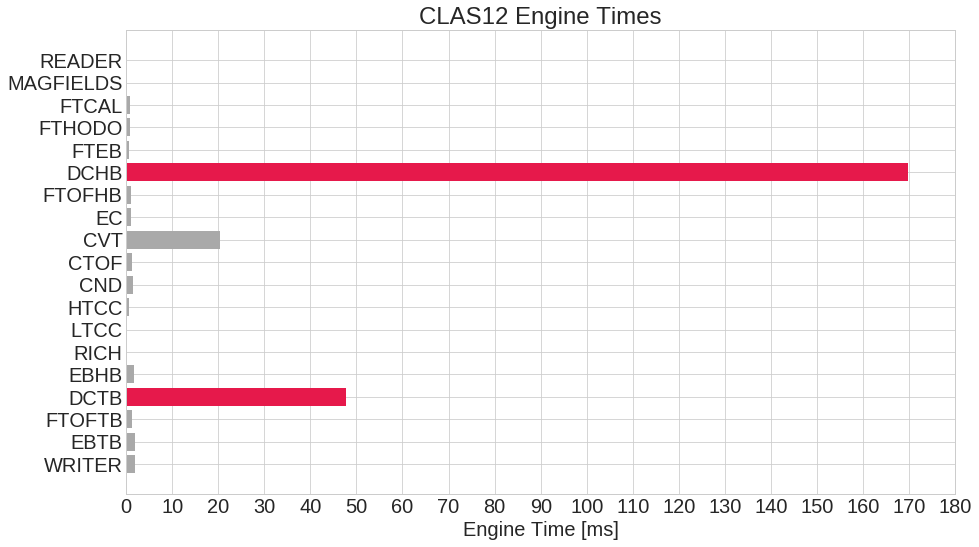
\includegraphics[scale=0.44]{methods_times/1_0.png}
    \caption{\label{fig:methods_times-1_0} Methods' CPU time on the original source code (version $1.0$).}
\end{figure}

\newpage

\subsection{Results} \label{ssec:prof_results}
Using the \textbf{jvisualvm} profiler, the time taken by each component of the CLAS12 offline software can be measured, thus finding the bottlenecks in the execution in order to prioritize work on them.
It's worth noting that all the profiled data presented in this publication is obtained via \textbf{jvisualvm} unless stated otherwise, running the CLAS12 software on $10.000$ events with real experimental data taken from the test file \texttt{clas\_004013.0.hipo}.

As a note before continuing, all figures that relate to profiling information will be always associated to a ``version''.
This is different from the versioning system utilized in the CLAS12 offline software, and is instead one used only in this work to quickly refer to different states of the software after each improvement, and thus, ``version $1.0$'' refers to the initial state of the code, before any changes are made by the author.

The methods taking up more than $2\%$ of the total CPU time before any change is made on the source code is shown in Figure \ref{fig:methods_times-1_0}.
A brief description of the methods in the figure are:

\begin{itemize}
    \item \textbf{Runge Kutta 4}: named \texttt{RK4transport} from the \texttt{RungeKutta} (\texttt{RK4} in Figure \ref{fig:methods_times-1_0}) class, the method is a direct implementation of the algorithm described in Section \ref{ssec:framework_rk4}, taking up a total of $35.1\%$ ($764.34$ seconds) of the total computation time.
    As is explained in detail in Section \ref{ssec:prop_magfield}, most of the time used in this method is taken up by a method to obtain the magnetic field at specific points.
    
    \item \textbf{Cluster Splitter}: named \texttt{clusterSplitter} from the \texttt{CCU} class, which is short for \texttt{ClusterCleanerUtilities}.
    As the name suggests, it refers to the process of splitting the clusters described in Section \ref{ssec:framework_cf} done via the Hough transform, which in simple terms consists of finding line shaped sub-clusters in the split cluster~\cite{hough1962method} and is described in detail in Appendix \ref{add:hough_transform}.
    
    The process is useful because it splits malformed clusters with poor performance to ones that are better fit, but, as can be seen in Figure \ref{fig:methods_times-1_0}, takes $22.4\%$ ($486.26$ seconds) of the total CPU time.
    This is attributed to the fact that it transforms every hit in the original cluster to a so-called ``Hough Space'' to find the split clusters, which is a slow process due to the raw number of hits in each cluster and the number of clusters.

    \item \textbf{Set Fit Array}: named \texttt{setFitArray} from the \texttt{ClusterFitter} (\texttt{CF} in the Figure) class, the method receives clusters and creates arrays from the hits in them which are later fit into a line by the \texttt{fitCluster} method from the same class.
    While the algorithm itself involves only sorting the cluster and then adding them to arrays, the method takes so much time ($18.2\%$ or $394.97$ seconds of the total CPU time) because it's called several times by many methods, especially the \texttt{findHitBasedClusters} method in the \texttt{ClusterFinder} class, and it sorts the cluster for each of these calls.
    
    \item \textbf{Is Nonsingular}: named \texttt{isNonsingular} from the class \texttt{KFitter} (\texttt{KF} in Figure \ref{fig:methods_times-1_0}), it's a method that returns \texttt{true} if a matrix is nonsingular and \texttt{false} otherwise, taking up a total of $10.2\%$ ($223.02$ seconds) of the total computation time.
    The method takes up this much time because it is called twice every time the \texttt{filter} method is called to check if the covariance matrix is singular, and it calculates the determinant of the matrix to do this.
    It's acceleration is discussed in detail in Section \ref{ssec:prop_matrices}.

    \item \textbf{Get Track Initial Fit}: named \texttt{getTrackInitFit} from the \texttt{TCLF} class, short for \texttt{TrackCandListFinder}.
    The method simply provides an initial fit to the Kalman Filter from which to start working, but it takes a total of $3.8\%$ ($82.34$ seconds) mainly due to lack of good programming practices.
    As can be seen later in Section \ref{ssec:val_refactoring_and_optimizations}, the method's time was lowered by a large factor simply by refactoring and applying simple optimizations to the code.
    
    \item \textbf{Calculate Trajectory}: named \texttt{calcTrajectory} from the \texttt{Trajectory} class (\texttt{Traj} in the Figure), this method receives a set of parameters from a track's state vector and, as the name suggests, it calculates and returns an estimated trajectory that the particle described by the vector could take.
    The method's time of $2.8\%$ ($60.42$ seconds) is attributed to the fact that it's ran many times in the code.
    
    \item \textbf{Filter}: represented by the \texttt{filter} method in the \texttt{KFitter} class, it's an implementation of the filtering component of the Kalman filter, described in detail in Section \ref{ssec:framework_ekf}.
    It takes in total of $2.8\%$ ($60.28$ seconds) of the CLAS12 CPU time and its acceleration is described along with the one for \texttt{isNonsingular} in Section \ref{ssec:prop_matrices}.
\end{itemize}

It is worth noting that to obtain the measurements given in this section, the CLAS12 code was profiled in \textbf{jvisualvm} via statistical sampling with a sampling period of $100$ [ms] and by profiling only the packages related to the Drift Chambers (DC): \texttt{org.jlab.service.dc} and \texttt{org.jlab.rec.dc}.
This was done to shorten the profiling sessions time by focusing only on the DC code.